% Vector diagram built at the manuscript width, 372 TeX points.
\documentclass[border=0pt]{standalone}
\usepackage[T1]{fontenc}
\usepackage{helvet}
\usepackage{tikz}
\usepackage{amsmath}
\usetikzlibrary{arrows.meta,positioning,fit,calc,backgrounds}
\definecolor{orxblue}{HTML}{0072B2}
\tikzset{
 orx/.style={font=\sffamily\fontsize{8.5}{10.5}\selectfont,>={Stealth[length=4pt,width=3pt]},line width=.5pt,node distance=8mm and 7pt},
 block/.style={draw=black!40,fill=white,rounded corners=1pt,align=center,inner sep=5pt},
 flow/.style={->,draw=black!60},
 diagnostic/.style={flow,dashed},
 edgelbl/.style={font=\sffamily\fontsize{8}{9.5}\selectfont,fill=white,inner sep=2pt,text=black!65},
 stage/.style={draw=black!25,fill=black!2,rounded corners=2pt,inner sep=7pt},
 stagelbl/.style={font=\sffamily\bfseries\fontsize{8.5}{10.5}\selectfont,anchor=west},
 frozen/.style={block,draw=orxblue,fill=orxblue!7,line width=.7pt}
}
\begin{document}
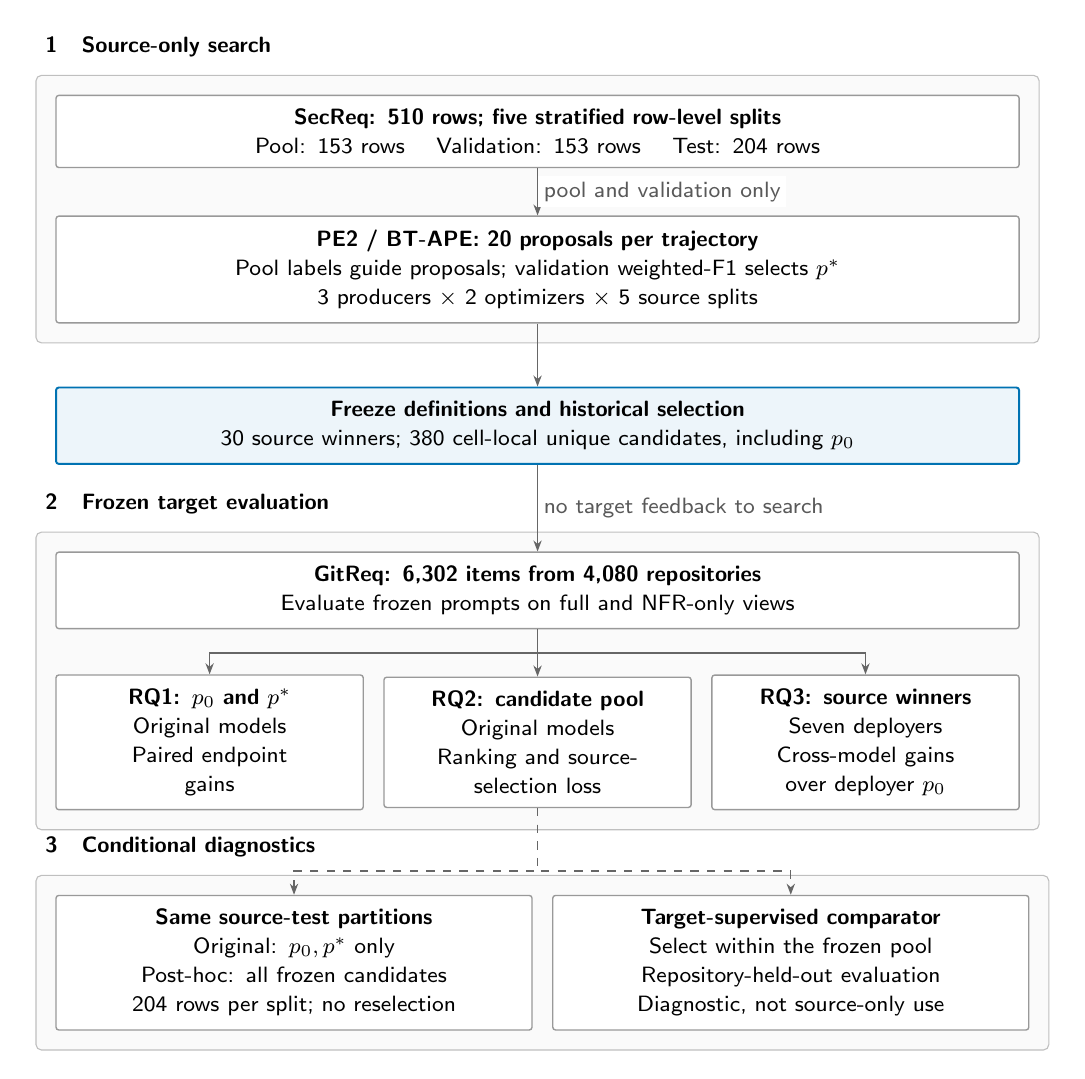
\begin{tikzpicture}[orx]
\node[block,text width=338pt] (source) {\textbf{SecReq: 510 rows; five stratified row-level splits}\\Pool: 153 rows \quad Validation: 153 rows \quad Test: 204 rows};
\node[block,text width=338pt,below=6mm of source] (search) {\textbf{PE2 / BT-APE: 20 proposals per trajectory}\\Pool labels guide proposals; validation weighted-F1 selects $p^*$\\3 producers $\times$ 2 optimizers $\times$ 5 source splits};
\draw[flow] (source) -- node[edgelbl,right] {pool and validation only} (search);
\begin{scope}[on background layer]
 \node[stage,fit=(source)(search)] (searchstage) {};
\end{scope}
\node[stagelbl,above=3pt of searchstage.north west,anchor=south west] {1\quad Source-only search};
\node[frozen,text width=338pt,below=8mm of search] (frozen) {\textbf{Freeze definitions and historical selection}\\30 source winners; 380 cell-local unique candidates, including $p_0$};
\draw[flow] (search) -- (frozen);
\node[block,text width=338pt,below=11mm of frozen] (target) {\textbf{GitReq: 6,302 items from 4,080 repositories}\\Evaluate frozen prompts on full and NFR-only views};
\node[block,text width=101pt,below=6mm of target] (rq2) {\textbf{RQ2: candidate pool}\\Original models\\Ranking and source-\\selection loss};
\node[block,text width=101pt,left=7pt of rq2] (rq1) {\textbf{RQ1: $p_0$ and $p^*$}\\Original models\\Paired endpoint\\gains};
\node[block,text width=101pt,right=7pt of rq2] (rq3) {\textbf{RQ3: source winners}\\Seven deployers\\Cross-model gains\\over deployer $p_0$};
\draw[flow] (frozen) -- node[edgelbl,right] {no target feedback to search} (target);
\draw[flow] (target.south) -- (rq2.north);
\draw[flow] (target.south) -- ++(0,-3mm) -| (rq1.north);
\draw[flow] (target.south) -- ++(0,-3mm) -| (rq3.north);
\begin{scope}[on background layer]
 \node[stage,fit=(target)(rq1)(rq3)] (evalstage) {};
\end{scope}
\node[stagelbl,above=3pt of evalstage.north west,anchor=south west] {2\quad Frozen target evaluation};
\node[block,text width=162pt,below=11mm of rq2,xshift=-88pt] (sourcetest) {\textbf{Same source-test partitions}\\Original: $p_0,p^*$ only\\Post-hoc: all frozen candidates\\204 rows per split; no reselection};
\node[block,text width=162pt,right=7pt of sourcetest] (targetchoice) {\textbf{Target-supervised comparator}\\Select within the frozen pool\\Repository-held-out evaluation\\Diagnostic, not source-only use};
\draw[diagnostic] (rq2.south) -- ($(rq2.south |- sourcetest.north)+(0,3mm)$) -| (sourcetest.north);
\draw[diagnostic] (rq2.south) -- ($(rq2.south |- targetchoice.north)+(0,3mm)$) -| (targetchoice.north);
\begin{scope}[on background layer]
 \node[stage,fit=(sourcetest)(targetchoice)] (diagnosticstage) {};
\end{scope}
\node[stagelbl,above=3pt of diagnosticstage.north west,anchor=south west] {3\quad Conditional diagnostics};
\node[fit=(searchstage)(evalstage)(diagnosticstage),inner sep=0pt,minimum width=372pt] (bounds) {};
\end{tikzpicture}
\end{document}
